\documentclass{article}
\usepackage[letterpaper,margin=1in]{geometry}
\usepackage{xcolor}
\usepackage{fancyhdr}
\usepackage{tgschola} % or any other font package you like
\usepackage{graphicx,subfigure, subcaption}
\usepackage[sorting=none]{biblatex} %Imports biblatex package

\addbibresource{reference.bib}

\def\system{RealityCanvas}
\pagestyle{fancy}
\fancyhf{}
\fancyhead[C]{%
  \footnotesize\sffamily
  \yourname\quad
  web: \textcolor{blue}{\itshape\yourweb}\quad
  \textcolor{blue}{\youremail}}

\newcommand{\soptitle}{Statement of Purpose}
\newcommand{\yourname}{Zhijie Xia}
\newcommand{\youremail}{zhijie.xia@ucalgary.ca}
\newcommand{\yourweb}{https://www.zhijiexia.dev/}

\newcommand{\statement}[1]{\par\medskip
  \underline{\textcolor{blue}{\textbf{#1:}}}\space
}

\usepackage[
  colorlinks=false,
  breaklinks,
  pdftitle={\yourname - \soptitle},
  pdfauthor={\yourname},
  unicode
]{hyperref}


\begin{document}

\begin{center}\LARGE\soptitle\\
\large \yourname\ , M.Sc Computer Science (Thesis), Robotics - Fall 2024
\end{center}

\hrule
\vspace{1pt}
\hrule height 1pt

\bigskip

I am writing to express my interest in pursuing a Master of Science in 
Computer Science (Thesis) with a focus on Robotics at McGill University.
Furthermore, I am excited about the prospect of becoming a member of the Mobile Robotics Lab.

My primary research interests lie in the areas of Deep Reinforcement Learning and Robot Control for applications.
I aspire to lead a robotic engineering team dedicated to constructing fully autonomous robots capable of addressing
real-world challenges.

My first experience with research occurred during an internship at the Programmable Reality Lab at University of Calgary 
after my third year of undergraduate studies. I was fascinated by sketching in AR as it is
a very intuitive way of creating virtual objects and wanted 
to make it more expressive and dynamic. 
My research interests were further developed when I worked on a research project with Dr. Ryo Suzuki. 
This was the "RealityCanvas" project, an authoring tool designed to facilitate the creation
of improvised scribble animation in an augmented environment~\cite{xia2023realitycanvas}.
I curated a dataset comprised of videos and images sourced from different social media platforms.
These contained scribble animations edited using context creation software like Adobe After Effects and Adobe Premiere Pro. 
This dataset served as the foundation for taxonomy analysis, in which I systematically catergorized
six animation techniques. Motivated by the taxonomy analysis,
I developed a web application that allows users to generate scribble animation using the six common techniques. 
Users can draw these animations directly onto the screen and apply them to the video stream. The workflow 
is shown shown in Figure \ref{fig:teaser}. In addition to designing and implementing the system, I conducted a user study to access its usability and expert
interviews to evaluate its effectiveness. The results of the user study demonstrated that the system facilitates
easy and spontaneous animation creation. Expert interviews further affirmed the system's effectiveness in generating 
scribble animations.

\begin{figure}[h!]
  \centering
  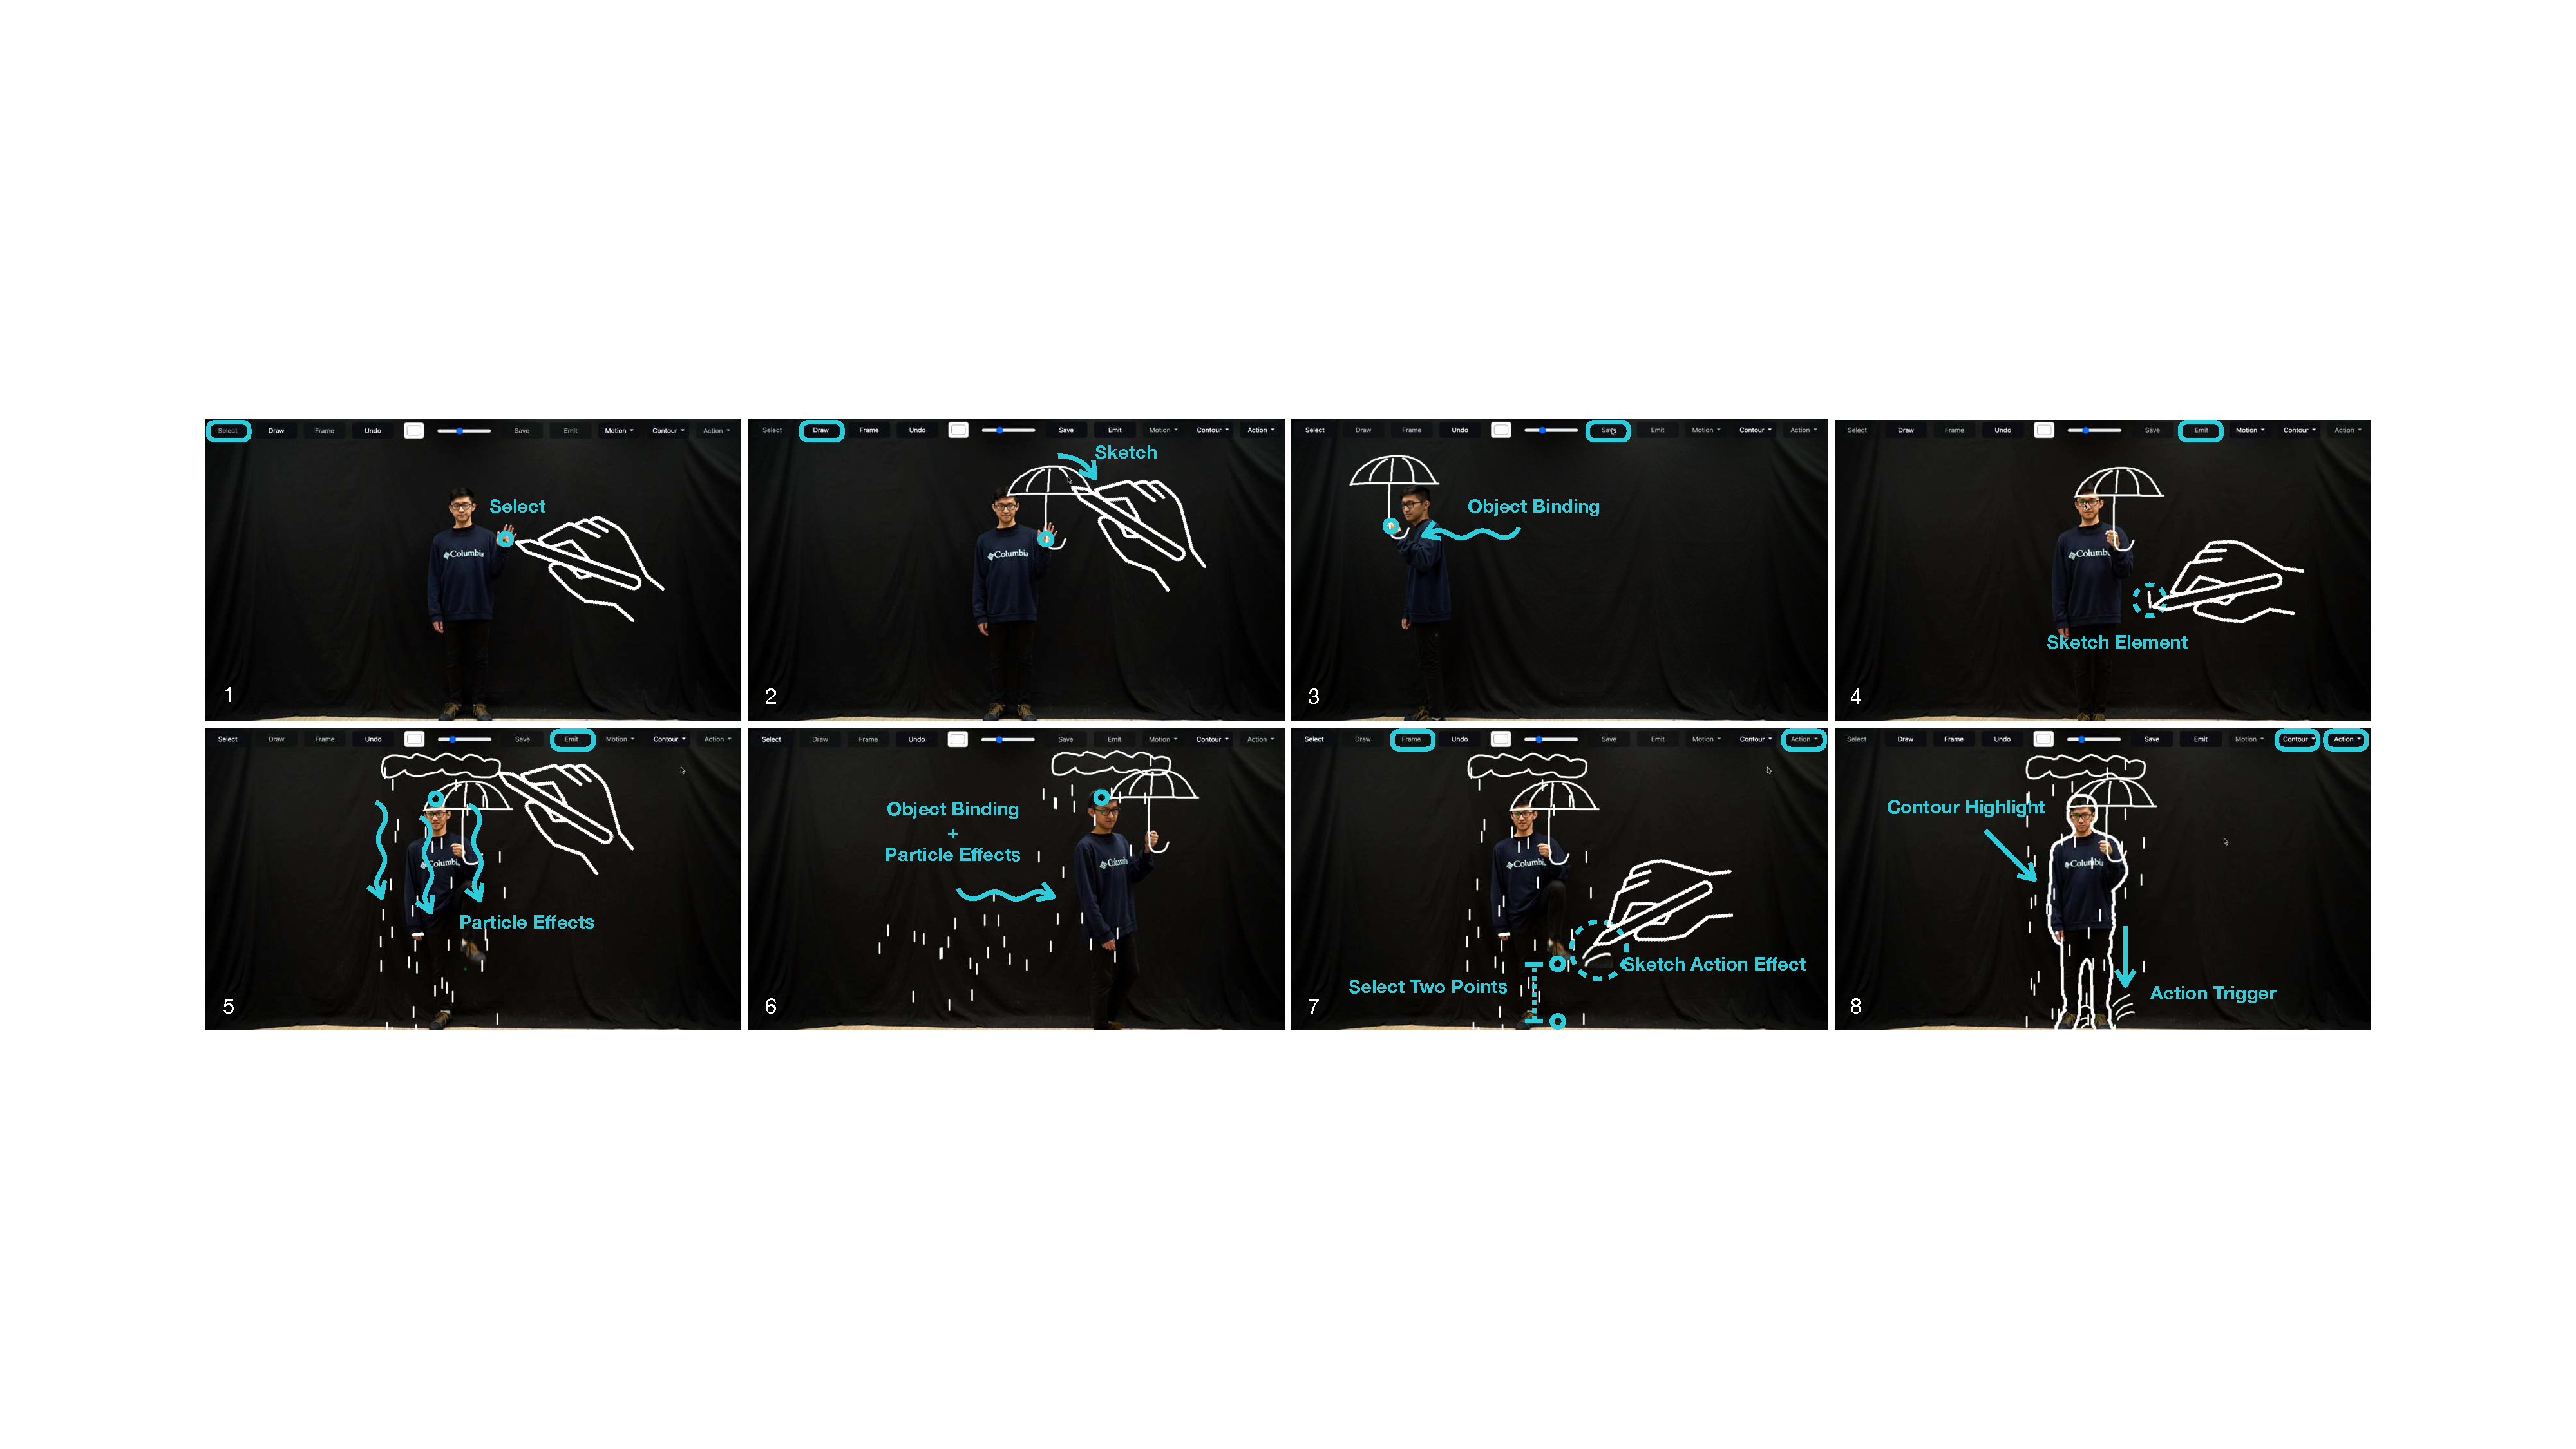
\includegraphics[width=\textwidth]{figures/teaser-num.pdf}
  \caption{\system{} workflow (from top left to bottom right): 1) select a hand as a tracking point, 2) sketch an umbrella bound to the hand, 3) the umbrella moves when the hand moves, 4) sketch a raindrop, 5) draw a cloud as an emitter line to show particle effects, 6) the cloud also moves with object binding, 7) select the ground and right foot then sketch a water splash, 8) show the water splash and contour highlight based on the stomp action.}
  \label{fig:teaser}
\end{figure}


During this internship, I have had the valuable opportunity to immerse myself in academic research, igniting my passion for 
applied research and computer science. I am deeply intrigued by the process of transforming ideas into real-world applications.
Working alongside Dr. Suzuki and his team, I came to realize that the world is constant state of flux, with perpetual challenges 
and uncharted ideas awaiting exploration. Even when addressing the same problem, there exist innovative approaches to tackle it, 
challenging established conventional solutions. During this internship, I navigated the entire academic research publication process, 
from conducting literature reviews and implementing the system to submitting the paper, 
addressing peer-review feedback, and achieving publication. 
The paper titled "RealityCanvas: Augmented Reality Sketching for Embedded and Responsive Scribble Animation Effects" [1], 
with me as the first author, was published at UIST 2023. This experience introduced me to academic research and fueled my enthusiasm 
for developing my research skills.


After completing my internship at the Programmable Reality Lab, I initiated an independent research project with Dr. Joel Reardon.
My undergraduate thesis revolved around an in-depth exploration of the Android permission system's design and implementation. 
My primary motivation for this research was to investigate the root causes of Android permission breaches 
and the significant prevalence of overprivileged apps.
The transition from Human-Computer Interaction (HCI) research to the field of security research presented both challenges and 
tremendous fullfillment. Drawing from my prior research experience, I applied my transferable research knowledge to this project. 
I conducted a comprehensive literature review and swiftly devised an approach by enhancing the state-of-the-art API 
permission mappings~\cite{felt2011android,au2012pscout}. Additionally, I implemented a pipeline for retrieving Android application APKs from the Google Play Store, 
decompiling them, extracting permission usage data, and mapping it to the corresponding API calls. 
Furthermore, I delved into various frequent itemset mining algorithms in pursuit of the optimal algorithm for 
mining permission usage patterns, ultimately selecting the FP-mining algorithm.

Our research revealed permission usage patterns for 35, 117 Android
applications we drawn from Google Play Store and we built a 
API-permission mapping with 1, 976 API calls and 323 permissions. We suspected that some of these patterns were malicious, 
leading us to conduct a manual analysis of our application corpus and the decompiled smali packages to
validate our concerns. Notably, we discovered applications that exploited the combination of \textit{$SET\_EXACT\_ALARM$} and 
\textit{$ACCES\_FINE\_LOCATION$} in our application corpus which periodically transmit device location data to servers. 
However, due to time constraints and personal challenges, we were unable to conduct a 
more extensive investigation of these potentially malicious applications and prepare them for the peer-review process.
This experience provided me with a robust introduction to the security domain and further enhanced my transferable skills 
for conducting independent research across diverse domains. It has intensified my determination to rectify
flaws and demand more from reality by aspiring to do and achieve more.


After joining Knowd AI, a venture-capital funded startup in Toronto, 
I focused on research and development for Knowd board, the company's flagship product.
Leveraging my previous work on "RealityCanvas," I designed an intuitive workflow for non-technical users, 
including drag-and-drop functionality, automatic clustering, and summarization features. 
I also improved the user interface for a more modern and user-friendly experience, 
informed by my research and user studies.
Furthermore, I conducted extensive research and integrated 
BERTopic~\cite{BERT} to support Knowd board's development, aligning 
with our MVP's requirements and contributing to its success. 
Currently, I'm a firmware developer at Lucid Vision Labs, Inc in Vancouver, 
where I transitioned from software to firmware development. This move reflects 
my desire for new challenges and expertise in camera systems and computer vision. 
My responsibilities include designing firmware for next-generation GigE cameras and 
developing a reporting suite for the manufacturing and testing team, expanding my industry expertise.


Throughout my journey, which spans from my undergraduate studies and research to my current 
industrial co-op experience, my determination and passion for pursuing academic research in graduate school 
have significantly intensified. I am drawn to the field of robotics for a profound reason: I envision a future 
where robots are not only ubiquitous but also indispensable in our daily lives. This vision has been a 
driving force since my early interest in robotics and my self study on the literature of deep reinforcement 
learning. I am motivated by the desire to create tangible 
solutions that can interact physically with the real world, rather than 
limiting my impact to SaaS products or mobile applications where only reside in virtual space.
I find various aspects of computer science fascinating, such as human-computer interaction, security, 
computer vision, and machine learning. The field of robotics stands out as particularly promising to me 
because it combines these interests and has the potential to make a significant real-world impact due to 
its multidisciplinary nature.


With the respect to my thesis, I am eager to collaborate under the guidance of 
Dr. Gregory Dudek, Dr. David Meger and/or Dr. Doina Precup's due to my deep interest in the projects undertaken by 
the Mobile Robotics Lab. Along with this, I find Dr. Gregory Dudek
and Dr. David Meger's work "Towards Autonomous Robotic Coral Reef Health Assessment"~\cite{manderson2016towards}
and "Learning to Drive Off Road on Smooth Terrain in Unstructured Environments Using an On-Board Camera and Sparse Aerial Images"~\cite{manderson2020learning}
particularly captivating that are examples of how robots can be used to solve real world problems in cross-disciplinary domains.
Dr. Doina Precup's work on "Deep reinforcement learning that matters"~\cite{henderson2018deep} is also of 
significant interest to me as it aligns with my values regarding the significance of reproducibility 
and the advancement of deep reinforcement learning research.

I would like to conclude with a quote from Dr. Ryo Suzuki's enlightening public talk at the Calgary Public Library:

"When the first messaging machine was invented in the latter part of the last century, people were astonished 
by a machine that could send messages. Then came the invention of the first mobile phone, 
and people marveled at a device that could transmit voice on a handheld gadget. Subsequently, 
the iPhone and the advent of so-called smartphones captivated us with machines we could touch. 
We have witnessed these profound changes. Nowadays, even six-year-olds instinctively touch every screen they encounter, 
assuming it to be touch-sensitive. In essence, we are all digital immigrants in a rapidly evolving world. We have a choice: 
embrace this change and contribute to making the world a better place, or ignore it and risk being left behind."

For me, the choice is clear—I choose to wholeheartedly embrace this change.
Beyond mere acceptance, my unwavering commitment lies in addressing the flaws within our world 
and tirelessly working towards crafting tangible solutions.
My focus centers on the development of autonomous robotics systems with the capacity to 
drive substantial impact. Simultaneously, I am determined in pushing the boundaries of what is 
achievable in our physical reality. Through these efforts, I aspire to make a meaningful contribution 
to the progress of our global community as a dedicated graduate researcher in the field of robotics.

% By admitting me, you will be adding a passionate and dedicated researcher to your program who has strong 
% research experience and a proven track record of success. I am confident that I will be a valuable addition
% to the Mobile Robotics Lab and look forward to the opportunity to contribute to the lab's research efforts.
% Aforemost, I am excited to collaborate with the lab's faculty and students to advance the field of robotics
% and make a meaningful contribution to the global community.

\printbibliography
\end{document}
